\begin{flushright} {\tiny {\color{gray} python\_codes/fieldstone\_117/text.tex}} \end{flushright}

\lstinputlisting[language=bash,basicstyle=\small]{python_codes/fieldstone_117/keywords}

\begin{center}

\fbox{\textbf{\huge \color{teal} P}}
Codes at \url{https://github.com/cedrict/fieldstone/tree/master/python_codes/fieldstone_01}
\end{center}

\par\noindent\rule{\textwidth}{0.4pt}

{\sl This fieldstone was developed in collaboration with Lukas van de Wiel}. \index{contributors}{L. van de Wiel}

\par\noindent\rule{\textwidth}{0.4pt}
%%%%%%%%%%%%%%%%%%%%%%%%%%%%%%%%%%%%%%%%%%%%%%%%%%%%%%%%%%%%%%%%%%%%%%%%%%%%%%%%%%%%%%%%%%%%%%

This is work in progress. There is still much to do. The idea here is to compare the 
accuracy of quads on a specific benchmark (SolVi) as obtained on a bespoke mesh.

%-------------------------------
\subsection*{The mesh}

The mesh(es) used in this \stone are obtained by means of the quilt mesher program written by Lukas. 

INSERT HERE MANUAL


In order to generate the meshes that the \stone needs, we need to modify two files:
\begin{itemize}
\item {\tt quilt.f}: elementType = Q0, Q1, Q2, Q3, or Q4
\item {\tt examples.f}: in subroutine meshThirteenPatches: nElemsBase=10
\end{itemize}

WARNING! As of now the edges of the elements are straight, so that the mid-egde nodes do not 
follow the curvature of the inclusion.

%-------------------------------
\subsection*{The benchmarks}

I have implemented five finite element pairs: $Q_1\times P_0$, $Q_2\times Q_1$, $Q_2 \times P_{-1}$
(both mapped and unmapped flavours), $Q_3\times Q_2$, $Q_4\times Q_3$. 
Note that unfortunately the vtu format does not allow the representation of $Q_3$ or $Q_4$ fields. 
The basis functions for all these elements are to be found in Section~\ref{sec:shpfct2d}.

Two benchmarks are implemented in the code: Donea \& Huerta (see Section~\ref{mms1}) and 
SolVi (see Section~\ref{ss:solvi}).
The first one is a manufactured solution which has a vertical and horizontal symmetry. 
As such the tailored mesh is of no use here. The second is of course why the mesher 
was developed in the first place: the viscosity contrast between 
inclusion and matrix aligns exactly with the mesh:

\begin{center}
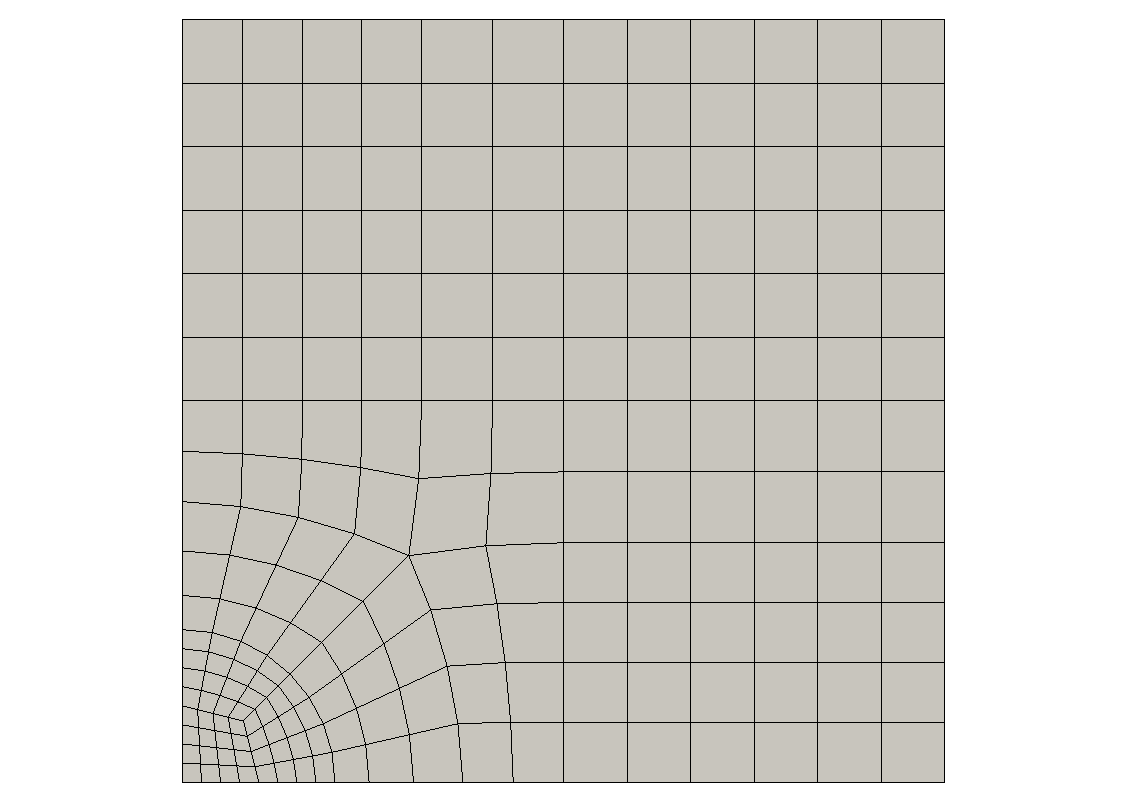
\includegraphics[width=5cm]{python_codes/fieldstone_117/images/mesh04}
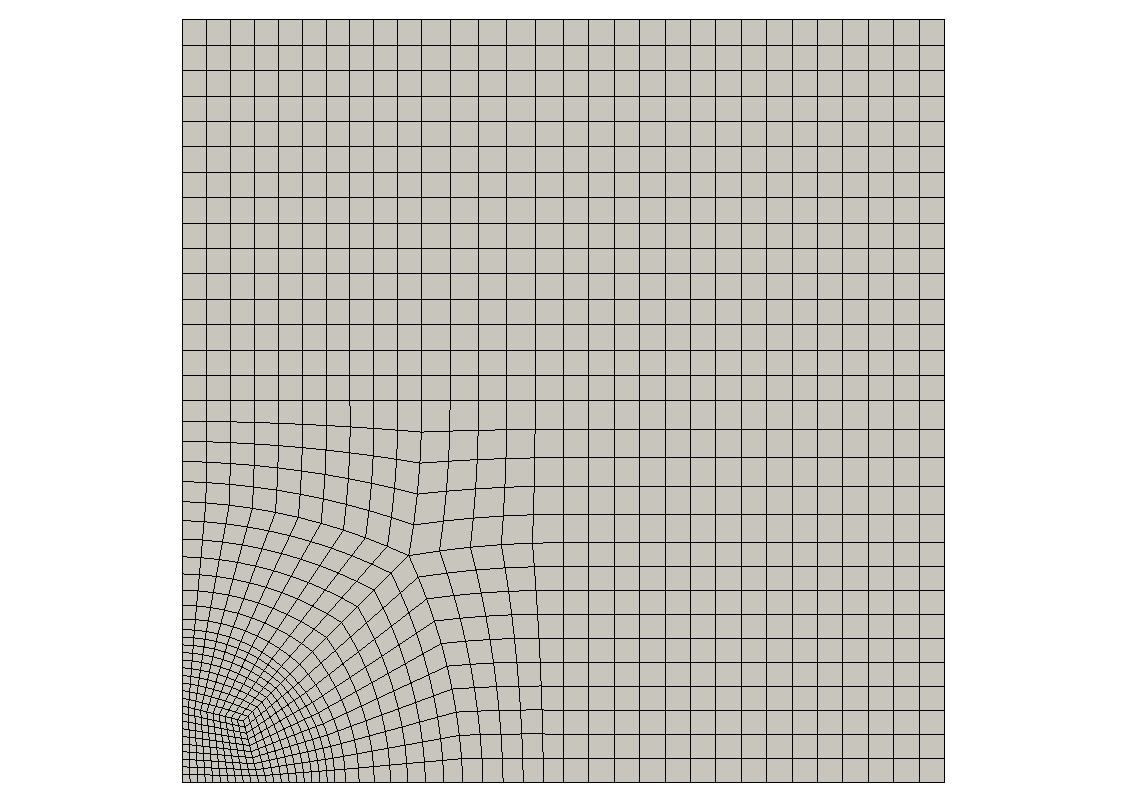
\includegraphics[width=5cm]{python_codes/fieldstone_117/images/mesh10}
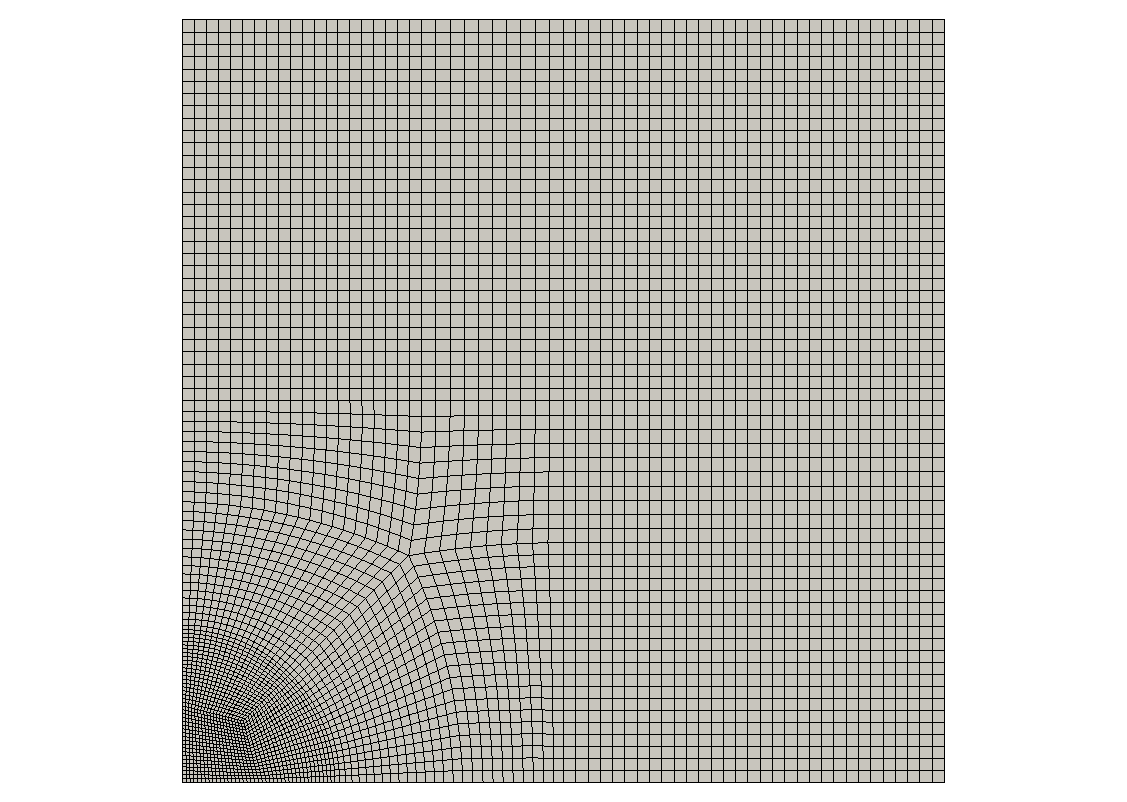
\includegraphics[width=5cm]{python_codes/fieldstone_117/images/mesh20}\\
{\captionfont Mesh generated with nElemsBase=4,10,20.}
\end{center}

\begin{center}
\begin{tabular}{ll}
\hline
{\tt element} & FE pair \\
\hline
\hline
1& $Q_1 \times P_0$ \\
2& $Q_2 \times Q_1$ \\
3& $Q_3 \times Q_2$ \\
4& $Q_4 \times Q_3$ \\
5& $Q_2 \times P_{-1}$ (mapped)\\
6& $Q_2 \times P_{-1}$ (unmapped)\\
\hline
\end{tabular}
\end{center}

manifold for viscosity interface?

do Q2(8)Q1


\begin{center}
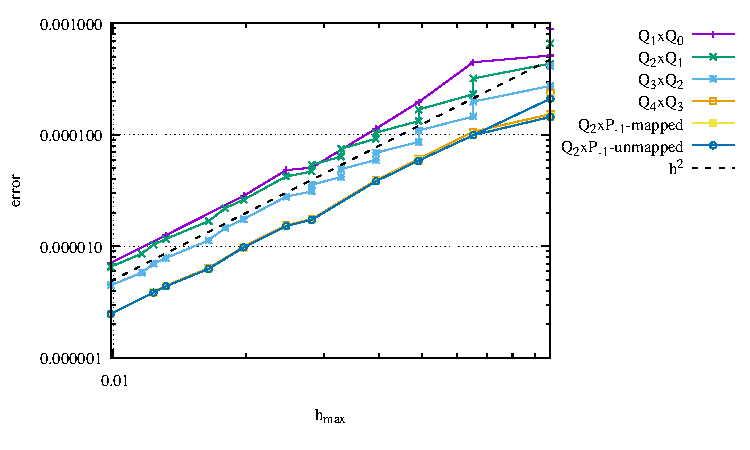
\includegraphics[width=7.5cm]{python_codes/fieldstone_117/results/errorsV}
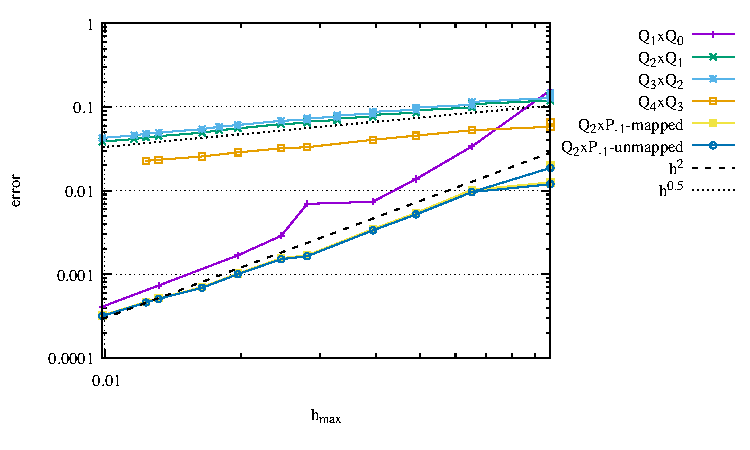
\includegraphics[width=7.5cm]{python_codes/fieldstone_117/results/errorsP}\\
{\captionfont SolVi benchmark: Velocity and pressure errors as a function of the largest element size in the mesh.}
\end{center}

include figure of p at bottom
